% Chapter Template

\chapter{Quadrotor Dynamic Model} % Main chapter title

\label{Chapter3} % Change X to a consecutive number; for referencing this chapter elsewhere, use \ref{ChapterX}

\lhead{Chapter 3. \emph{Quadrotor Dynamic Model}} % Change X to a consecutive number; this is for the header on each page - perhaps a shortened title

%----------------------------------------------------------------------------------------
%	SECTION 1
%----------------------------------------------------------------------------------------

In this chapter, a mathematical model of the quad-rotor is derived, and the assumptions that go into this derivation are explained in detail. This model will be used as the basis for the optimization techniques outlined in subsequent chapters.

\section{Description of a quad-rotor}

A generic model of a quad-rotor is physically composed of a simple frame supporting four brush-less motors. Thrust is provided by propellers attached to these motors. The speeds of the rotors are governed by a control algorithm which is implemented on some form of on board processor.

 The stabilization and control of a quad-rotor is accomplished by varying the speeds of the motors. The thrust the in vertical direction is controlled by varying all four motor speeds uniformly. In the quad-rotor frame of reference, the direction of the thrusts from the motors is fixed. This means that in order to produce lateral motion, the UAV must tilt such that a component of the total thrust vector points in the desired direction of motion. The pitch and roll angular positions are controlled by driving motors on opposite sides of the frame at different speeds. This produces torque about the center of mass of the quad-rotor. Given non-zero pitch, roll, and total thrust, the UAV experiences horizontal linear acceleration. The yaw angular position is controlled by driving pairs of opposite motors at the different speeds. This produces a torque about the yaw axis but not about the pitch or roll axes. Also, the two opposite pairs of motors must spin in opposite directions so that when hovering, the net torque about the yaw axis is zero. The details of this description are represented mathematically in the next section.



\section{Coordinate System Definitions}

In order to implement a control algorithm, we must understand the mathematical relationships between the control input and the resulting dynamics of the system. Using the Euler-Lagrange formulation from classical mechanics, we can obtain a nonlinear, deterministic dynamical model. General derivation of the Euler Lagrange differential equations of motion can be found in \cite{marion1995classical} and  \cite{cornelius1970variational}.

 The linear and angular coordinates are defined as follows. in Figure \ref{fig:quad-rotor coordinate system} the basic mechanical structure and the relationships between the spatial coordinates are shown.

\begin{figure}[htbp]
	\centering
		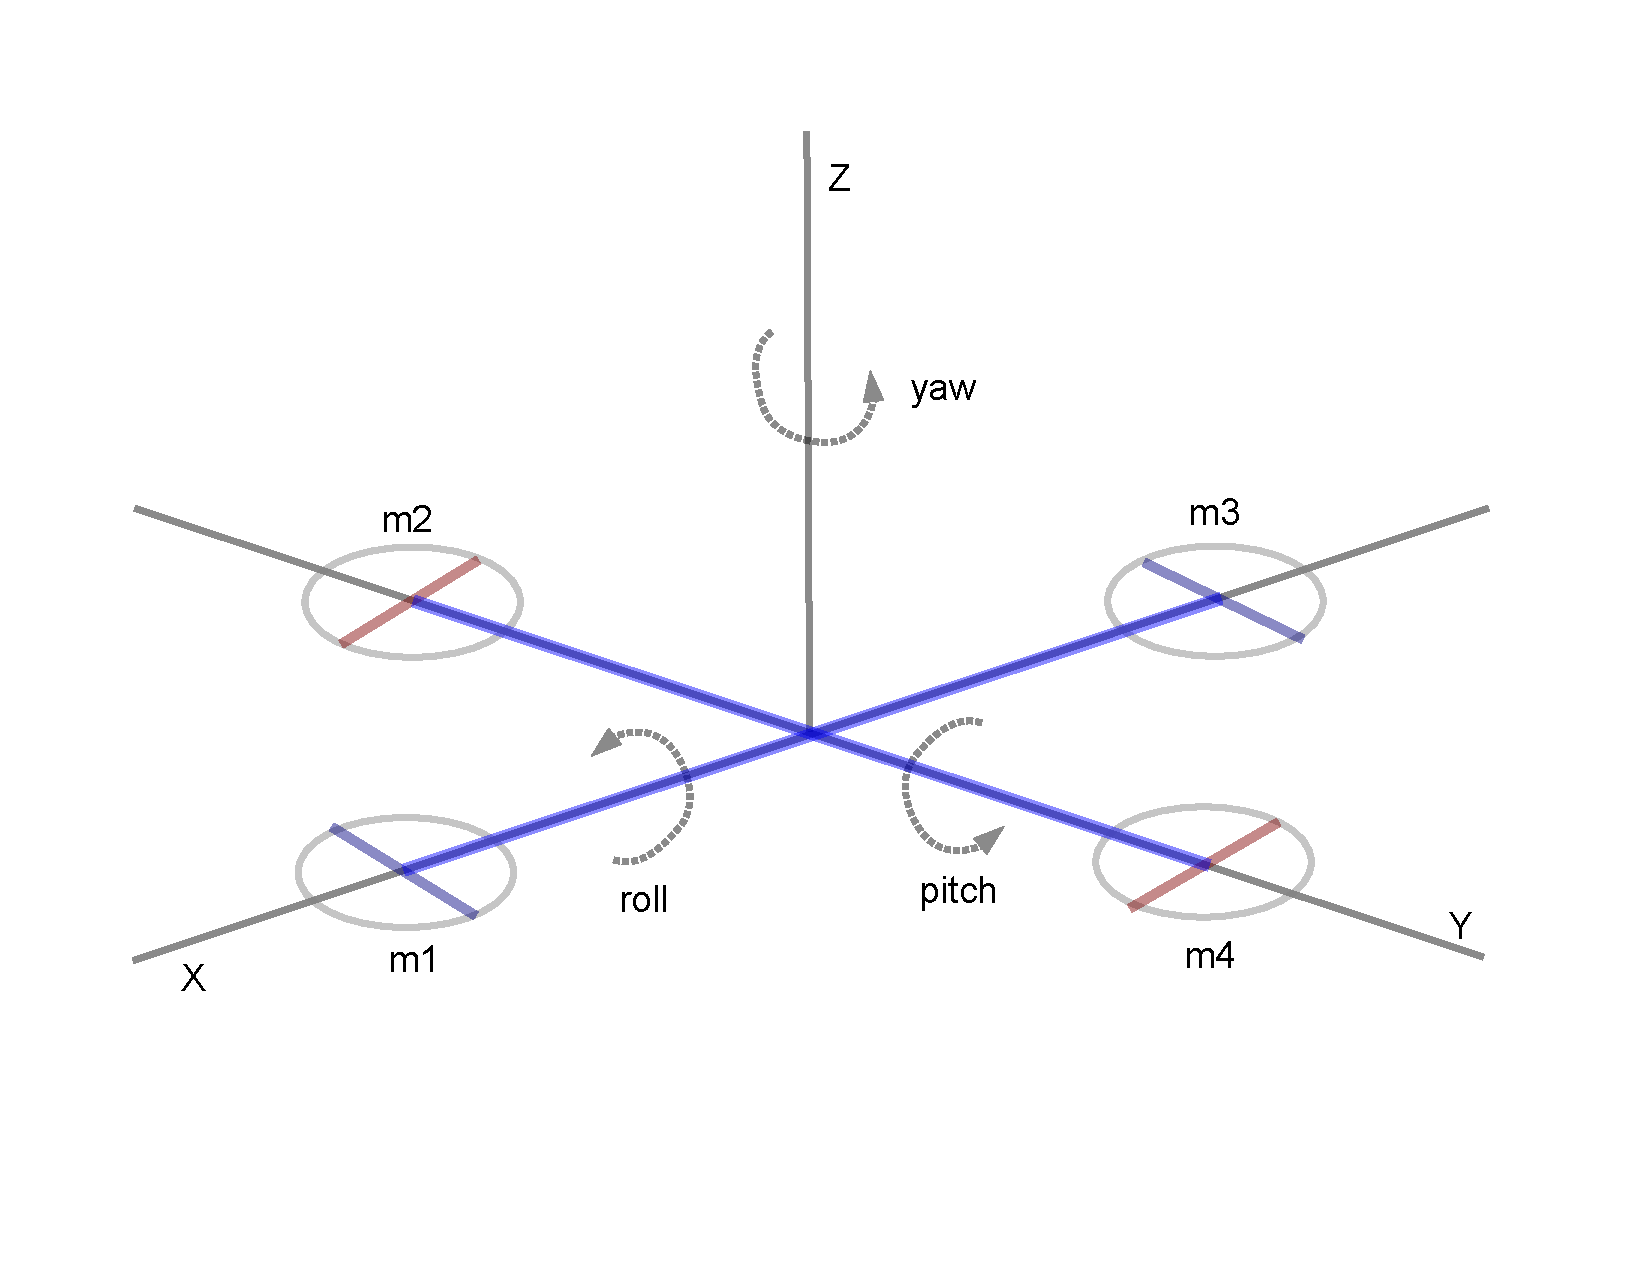
\includegraphics[width=\textwidth]{Figures/coords.pdf}
		\rule{35em}{0.5pt}
	\caption[quad-rotor coordinate system]{quad-rotor coordinate system}
	\label{fig:quad-rotor coordinate system}
\end{figure}


\indent $ \psi $ is the yaw angle around the z-axis\\
\indent $ \theta $ is the pitch angle around the y-axis\\
\indent $ \phi $ is the roll angle around the x-axis\\

The spatial variables can be grouped into linear and angular components.

$\boldsymbol \xi = \left[ \begin{array}{c}
x\\y\\z\\
\end{array} \right] $, $\boldsymbol \eta =  \left[ \begin{array}{c}
\phi\\\theta\\\psi\\
\end{array} \right] $, $\boldsymbol q = \left[ \begin{array}{c}
\xi\\\eta\\
\end{array} \right]$\\


\section{Motor Speeds, Thrust and Torque}

\indent The rotor angular velocities are related to the forces they produce by $f_i = k \omega^2_i$ where $k$ is the constant of proportionality.
The torques due to the rotors about the rotors' axes of rotation are given by $\tau_{M_i} = b \omega^2_i + I_M \dot{\omega}_i$. The parameter b is a drag coefficient. Note the effect of $\dot{\omega}_i$ is considered to be negligible because the rotational inertia of the rotor itself is negligible.

In the quad-rotor frame of reference, the motors produce torques on the system.

\begin{equation}
    \label{taub}
    \boldsymbol \tau_B = \left[ \begin{array}{c} \tau_{\phi}\\\tau_{\theta}\\\tau_{\psi}\\ \end{array} \right] = \left[ \begin{array}{c} l s (-\omega_2^2 + \omega_4^2)\\l s (-\omega_1^2 + \omega_3^2)\\ \displaystyle \sum \limits_{i=1}^4 b \omega^2\\\end{array} \right]
\end{equation}

The combined thrust of the rotors in the direction of the quad-rotor frame $z$ axis is\\

$\boldsymbol T_B = [0, 0, T]^T$ where,\\

\begin{equation}
    \label{totalThrust}
    T =  \displaystyle \sum \limits_{i=1}^4 f_i
\end{equation}.



\section{Euler-Lagrange Equations of Motion}


\noindent 
The mass of the quad-rotor is $m$. Each of the moments of inertia  $ i_{xx} $  and $ i_{yy} $
are assumed to be composed of a rod of length $ L $   which accounts for half of the mass of the quad-rotor. Assume the mass
is evenly distributed along the two perpendicular rods. Let  \(\beta  =\text{  }\frac{1}{12}m l^2 \). The inertia matrix for the quad-rotor is then: \\

\begin{equation}
I = \left(
\begin{array}{ccc}
 \frac{1}{12}\left(\frac{m}{2}\right)l^2 & 0 & 0 \\
 0 & \frac{1}{12}\left(\frac{m}{2}\right)l^2 & 0 \\
 0 & 0 & \frac{1}{12}m l^2 \\
\end{array}
\right) = \left(
\begin{array}{ccc}
 \frac{\beta }{2} & 0 & 0 \\
 0 & \frac{\beta }{2} & 0 \\
 0 & 0 & \beta  \\
\end{array}
\right).
\end{equation}

\noindent In the inertial frame, the kinetic and potential energy of the system are given by

%translational kinetic energy
\begin{equation}
    T_{\text{trans}}=\frac{1}{2}m\dot{\xi }^T\dot{\xi }
\end{equation}


%rotational kinetic energy
\begin{equation}
    T_{\text{rot}}= \frac{1}{2}\dot{\eta }^T J \dot{\eta } 
\end{equation}


% system potential energy
\begin{equation}
    U = m g z.
\end{equation}


The Lagrangian is formed as the difference between kinetic and potential energy.

\begin{equation}
    L = \frac{1}{2}m\dot{\xi }^T\dot{\xi }+\frac{1}{2}\dot{\eta }^T   J   \dot{\eta }\text{  }- m g z
\end{equation}

The Jacobian $J$, is given by

\begin{equation}
    J = W_{\eta}^T I W_{\eta} 
\end{equation} .

\begin{equation}
 W_{\eta} = \left[ \begin{array}{ccc}

1 & 0 & -sin(\theta)\\ 0 & cos(\phi) & cos(\theta) sin(\phi)\\ 0 & -sin(\phi) & cos(\theta) cos(\phi)\\

\end{array} \right]
\end{equation}



\noindent The matrix $ W_{\eta}$ is the matrix transformation which relates the angular velocities from the quad-rotor frame of reference to the inertial frame.



\begin{equation}
\label{J}
J= \left(
\begin{array}{ccc}
 \frac{\beta }{2}    & 0                                                                    & -\frac{\beta }{2}s(\theta) \\
 0                   & \frac{\beta}{2} c(\phi)^2 + \beta s(\phi)^2                       & \frac{- \beta}{2} c(\phi) \text{ } s(\phi) \text{ } c(\theta)  \\
 -\beta s(\theta)   & \frac{- \beta}{2} c(\phi) \text{ } s(\phi) \text{ } c(\theta)    & \frac{\beta }{2}s(\theta)^2 + \frac{\beta }{2} s(\phi)^2  c(\theta)^2 + \beta  c(\phi)^2  c(\theta)^2  \\
\end{array}
\right)
\end{equation}




\noindent The dynamics of the system are represented by the Euler - Lagrange differential equations of motion.

\begin{equation}
    \frac{d}{\text{dt}} \left( \frac{\delta  L} {\delta \dot{q}}\right) - \frac{\delta  L}{\delta q}=F 
\end{equation}


$ q = \{x,y,z,\psi ,\theta ,\phi \} = \{ \xi , \eta \}  $.


\noindent  $ f $ is the generalized force vector representing the linear external force acting on the system. 
$\tau $ is the vector of torques acting on the system due to the rotors.

\begin{equation}
    \left( \begin{array}{c} f \\ \tau \\ \end{array} \right) = \frac{d}{\text{dt}} \left( \frac{\delta  L} {\delta \dot{q}}\right) - \frac{\delta  L}{\delta q}
\end{equation}

General derivations of the Euler-Lagrange equations of motion can be found in \cite{marion1995classical} and  \cite{cornelius1970variational}. 

The coordinates  $ q_i=\{x,y,z,\psi ,\theta ,\phi \} $  are in reference to a ground based inertial coordinate system. The system states and control inputs must be mapped from the quad-rotor frame of reference to the inertial frame in order to express the dynamics of the system. The matrix below represents an arbitrary rotation transformation from the body frame to the inertial frame is:

\begin{equation}
\boldsymbol R = \left[ \begin{array}{ccc}
c(\psi) c(\theta) & c(\psi) s(\theta) s(\phi) - s(\psi) c(\phi) & c(\psi) s(\theta) c(\phi) + s(\psi) s(\phi)\\
s(\psi) c(\theta) & s(\psi) s(\theta) s(\phi) + c(\psi) c(\phi) & s(\psi) s(\theta) c(\phi) - c(\psi) s(\phi)\\
-s(\theta) & c(\theta) s(\phi) & c(\theta) c(\phi)\\
\end{array} \right]\\
\end{equation}

For simplicity, cos is denoted by 'c' and sin is denoted by 's' in the above expression. 





\noindent The linear components of the generalized forces produce the following equations.

\begin{equation}
    \label{linforce}
    f =  R  T_B = m \ddot{ \xi} -  G
\end{equation}


\begin{equation}
    m\left(\begin{array}{c}
      \ddot{x}\\
      \ddot{y}\\
      \ddot{z}\\
    \end{array}\right)
    - \left( \begin{array}{c}
        0\\
        0\\
        -m g  
      \end{array} \right)
      =u
     \left(
    \begin{array}{c}
     \cos{\psi}\sin{\theta}\cos{\phi} + \sin{\psi}\sin{\phi} \\
     \sin{\psi}\sin{\theta}\cos{\phi} - \cos{\psi}\sin{\phi} \\
     \cos{\theta} \cos{\phi} \\
    \end{array}
    \right)
\end{equation}


\noindent The angular components are expressed as

\begin{equation}
    \tau = \tau_b =\frac{d}{dt} \left( \frac{\partial  L} {\partial \dot{\eta}}\right) - \frac{\partial  L}{\partial \eta}
\end{equation}

\begin{equation}
    \tau_b =\frac{d}{dt} ( J \dot{\eta} ) - \frac{1}{2} \frac{\partial}{\partial \eta} ( \dot{\eta}^T J \dot{\eta}  ) 
\end{equation}

\begin{equation}
    \tau_b =J \ddot{\eta} + \frac{d}{dt}(J) \dot{\eta} - \frac{1}{2} \frac{\partial}{\partial \eta} ( \dot{\eta}^T J \dot{\eta}  ) 
\end{equation}

\begin{equation}
    \tau_b =  J \ddot{\eta} + \cc(\eta,\dot{\eta}) \dot{\eta} 
\end{equation}

\begin{equation}
    \label{eq:angularacc}
    \ddot{\eta} = J^{-1} \big( \tau_b - \cc(\eta,\dot{\eta}) \dot{\eta} \big) 
\end{equation}


The Coriolis matrix is defined as follows. {\color{red} NEED A REFEREED DOCUMENT WITH THE DERIVATION}



\begin{equation}
\label{cor}
    \cc(\eta,\dot{\eta}) = 
    \left(
        \begin{array}{c c c}
            \cc_{(11)} & \cc_{(12)} & \cc_{(13)} \\
            \cc_{(21)} & \cc_{(22)} & \cc_{(23)} \\
            \cc_{(31)} & \cc_{(32)} & \cc_{(33)} \\
        \end{array}
    \right)
\end{equation}




$\cc_{(11)} = 0$

$\cc_{(12)}  = (I_{yy}-I_{zz})  ( \dot{\theta} C_{\phi} S_{\phi} +  \dot{\psi} C_{\theta} S_{\phi}^2 )  + (I_{zz}-I_{yy})  \dot{\psi} C_{\phi}^2 C_{\theta} - I_{xx}  \dot{\psi} C_{\theta}$


$\cc_{(13)} = (I_{zz}-I_{yy})    \dot{\psi}   C_{\phi}   S_{\phi}  C_{\theta}^2$


$\cc_{(21)} = (I_{zz}-I_{yy})   ( \dot{\theta} C_{\phi} S_{\phi} +  \dot{\psi} S_{\phi} C_{\theta} ) + (I_{yy}-I_{zz})    \dot{\psi}   C_{\phi}^2  C_{\theta} + I_{xx}    \dot{\psi}   C_{\theta}$


$\cc_{(22)}  = (I_{zz}-I_{yy}) \dot{\phi} C_{\phi} S_{\phi}$


$\cc_{(23)}  = -I_{xx}  \dot{\psi} S_{\theta} C_{\theta} + I_{yy}  \dot{\psi} S_{\phi}^2 S_{\theta} C_{\theta} + I_{zz} \dot{\psi} C_{\phi}^2 S_{\theta} C_{\theta}$


$\cc_{(31)} = (I_{yy}-I_{zz}) \dot{\psi} C_{\theta}^2 S_{\phi} C_{\phi} - I_{xx} \dot{\theta} C_{\theta}$


$\cc_{(32)}  = (I_{zz}-I_{yy}) ( \dot{\theta} C_{\phi} S_{\phi} S_{\theta} + \dot{\phi} S_{\phi}^2 C_{\theta} ) + (I_{yy}-I_{zz}) \dot{\phi} C_{\phi}^2 C_{\theta} + I_{xx}  \dot{\psi} S_{\theta} C_{\theta} - I_{yy}  \dot{\psi} S_{\phi}^2 S_{\theta} C_{\theta} - I_{zz}  \dot{\psi} C_{\phi}^2 S_{\theta} C_{\theta}$


$\cc_{(33)} = (I_{yy}-I_{zz})   \dot{\phi}  C_{\phi} S_{\phi} C_{\theta}^2 - I_{yy}   \dot{\theta} S_{\phi}^2 C_{\theta} S_{\theta} - I_{zz} \dot{\theta} C_{\phi}^2 C_{\theta} S_{\theta} + I_{xx} \dot{\theta} C_{\theta} S_{\theta}$\\



%-------------------------------------------------------------------------
 
In general, the Coriolis term is a mathematical result of the rotational motion of one coordinate system with respect to another. Since we are considering arbitrary three dimensional motion, there are three orthogonal axes of rotation and the resulting matrix is quite complicated. According to the expression for the angular acceleration (equation \eqref{eq:angularacc}), the physical units of the Coriolis term must be torque to maintain algebraic continuity. It is important to keep in mind that the Coriolis term does not represent a real force or torque acting on the system. It is only an artifact which is needed to account for the relative rotation of one coordinate frame with respect to another.   






\section {A Complete Model}


A complete mathematical representation of the quad-rotor is as follows.\\ 

\begin{equation}
    \label{lineareq}
    \left(
        \begin{array}{c}
           \ddot{x}\\
           \ddot{y}\\
           \ddot{z}\\
        \end{array}
    \right)
    = \left(
       \begin{array}{c}
        0\\
        0\\
        g  
      \end{array}
    \right)
    +\frac{T}{m}
     \left(
        \begin{array}{c}
             C_{\psi}S_{\theta}C_{\phi} + S_{\psi}S_{\phi} \\
             S_{\psi}S_{\theta}C_{\phi} - C_{\psi}S_{\phi} \\
             C_{\theta} C_{\phi} \\
        \end{array}
    \right)
\end{equation}

\begin{equation}
    \label{angulareq}
    \left(
        \begin{array}{c}
           \ddot{\phi}\\
           \ddot{\theta}\\
           \ddot{\psi}\\
        \end{array}
    \right) = J^{-1}
    \left[ \left(
        \begin{array}{c}
            l s (-\omega_2^2 + \omega_4^2)\\
            l s (-\omega_1^2 + \omega_3^2)\\ 
            \sum \limits_{i=1}^4 b \omega_i^2\\
        \end{array}
    \right) -
    \cc
    \left(
        \begin{array}{c}
           \dot{\phi}\\
           \dot{\theta}\\
           \dot{\psi}\\
        \end{array}
    \right)
    \right]
\end{equation}


This system model is admittedly rather involved and non-linear. Even in this form there are many important aspects of quadrotor flight dynamics and environmental variables which are omitted. The general problem of designing a system that is able to understand and adapt to varying goals and circumstances is a huge one. 

Despite the apparent shortcomings of this model, it is very useful as a core component to this thesis. Although the assumed mathematical environment is somewhat of a departure from really, it allows for a firm theoretical basis which validates the development of the control system and optimization scheme.





